% file: 3-9-connectivity/cut-edge-structure.tex

\documentclass[tikz]{standalone}
\usetikzlibrary{positioning, shapes, fit}

\begin{document}
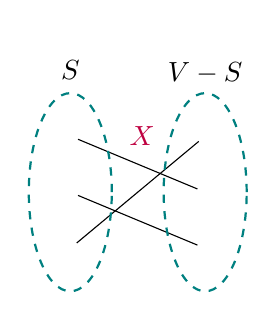
\begin{tikzpicture}[every node/.style = {draw, circle, inner sep = 2pt},
  node distance = 0.50cm and 1.5cm,
  comp/.style = {draw, thick, dashed, teal, ellipse, minimum height = 40pt, minimum width = 30pt}]
  \node (u1) [draw = none] {};
  \node (u2) [draw = none, below = of u1] {};
  \node (u3) [draw = none, below = of u2] {};

  \node (v1) [draw = none, right = of u1] {};
  \node (v2) [draw = none, below = of v1] {};
  \node (v3) [draw = none, below = of v2] {};

  \node (x) [draw = none, right = 0.50cm of u1, purple] {$X$};

  \path (u1) edge (v2)
  	(u2) edge (v3)
	(u3) edge (v1);

  \node [fit = (u1) (u2) (u3), comp, label = {[above] $S$}] {};
  \node [fit = (v1) (v2) (v3), comp, label = {[above = -10pt] $V - S$}] {};
\end{tikzpicture}
\end{document}
